% !TEX root = ../main.tex

\section{Results and discussion}

Characterization of the biomass along with batch reactor and sensitivity analysis results are discussed in this section.

\subsection{Blend3 biomass composition}

Several approaches were investigated to characterize the Blend3 feedstock for use with the Debiagi pyrolysis kinetics. The first approach uses the characterization method discussed in the Debiagi et al. 2015 paper where carbon and hydrogen from ultimate analysis is used to determine the biomass composition \cite{Debiagi-2015}. To use this approach for the Blend3 feedstock, the mass fraction of C and H on a dry ash-free basis (last column in Table \ref{tab:blend3-ult-bases}) is used for the biomass characterization procedure.

\begin{table}[H]
    \centering
    \caption{Ultimate analysis bases calculated from the Blend3 feedstock as-received data. Mass percent values are given for as-received (ar), dry, and dry ash-free (daf) basis.}
    \label{tab:blend3-ult-bases}
    \begin{tabular}{lrrrr}
        \toprule
        Element & \% ar & \% dry & \% daf & \% daf \\
        \midrule
        C        & 49.52 & 52.70 & 53.06 & 53.16 \\
        H        & 5.28  & 5.62  & 5.66  & 5.67  \\
        O        & 38.35 & 40.82 & 41.10 & 41.17 \\
        N        & 0.15  & 0.16  & 0.16  &       \\
        S        & 0.02  & 0.02  & 0.02  &       \\
        ash      & 0.64  & 0.68  &       &       \\
        moisture & 6.04  &       &       &       \\
        \bottomrule
    \end{tabular}
\end{table}

\textbf{Case 1:} The first approach to characterize the Blend3 feedstock was performed using a carbon mass fraction of 53.16\%, hydrogen mass fraction of 5.67\%, and splitting parameters $\alpha = 0.6$, $\beta = 0.8$, $\gamma = 0.8$, $\delta = 1.0$, and $\epsilon = 1.0$ which do not account for extractives in the feedstock. Results from this characterization are shown in Figure \ref{fig:blend3-biocharact-ult} and the associated biomass composition is given in Table \ref{tab:blend3-biocomp}. While this approach is useful for limited feedstock data, its accuracy is questionable when compared to experimental measurements. For example, chemical analysis of the Blend3 feedstock provides a lignin composition of 29.48\% (see Table \ref{tab:blend3-chem-analysis}) whereas the characterization method using ultimate analysis data estimates a total lignin composition greater than 59\%.

\begin{figure}[H]
    \centering
    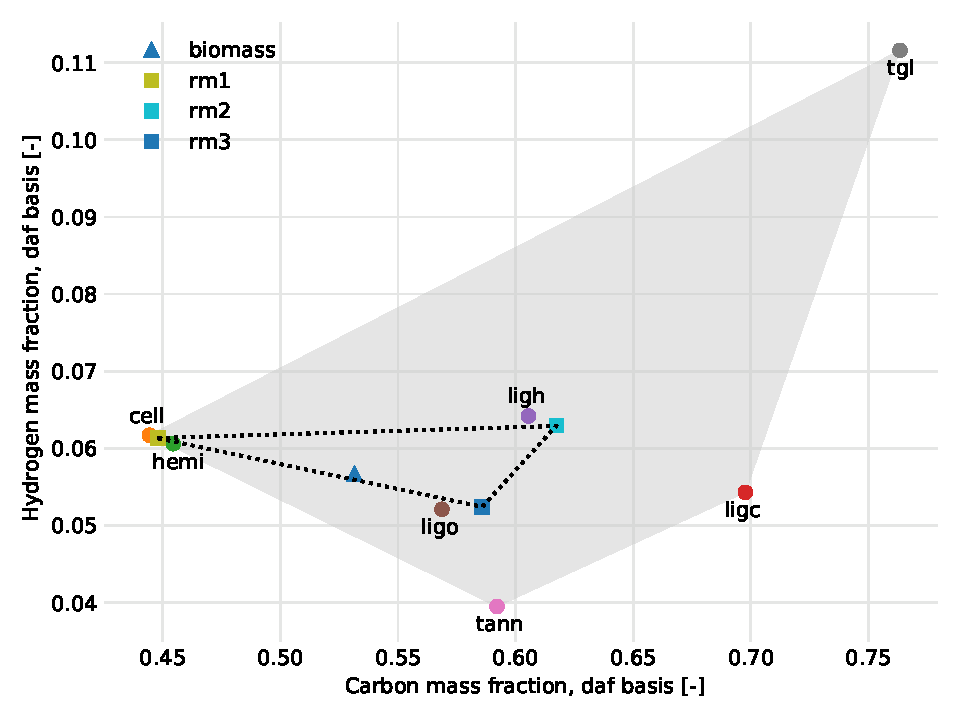
\includegraphics[width=0.8\textwidth]{figures/blend3-biocharact-ult.pdf}
    \caption{Characterization of the Blend3 feedstock using ultimate analysis data. Reference mixtures (rm) are labeled with square markers.}
    \label{fig:blend3-biocharact-ult}
\end{figure}

\textbf{Case 2:} To improve the Blend3 characterization based on ultimate analysis data, the splitting parameters were adjusted to account for extractives in the feedstock by using $\alpha = 0.56$, $\beta = 0.6$, $\gamma = 0.6$, $\delta = 0.78$, and $\epsilon = 0.88$. Also, since the uncertainty in the ultimate analysis data is unknown (see Table \ref{tab:blend3-ult}) the carbon mass fraction was adjusted to 51\% and the hydrogen mass fraction to 6\%. Results from these adjustments are presented in Figure \ref{fig:blend3-biocharact-ultmod} and Table \ref{tab:blend3-biocomp}.

\begin{figure}[H]
    \centering
    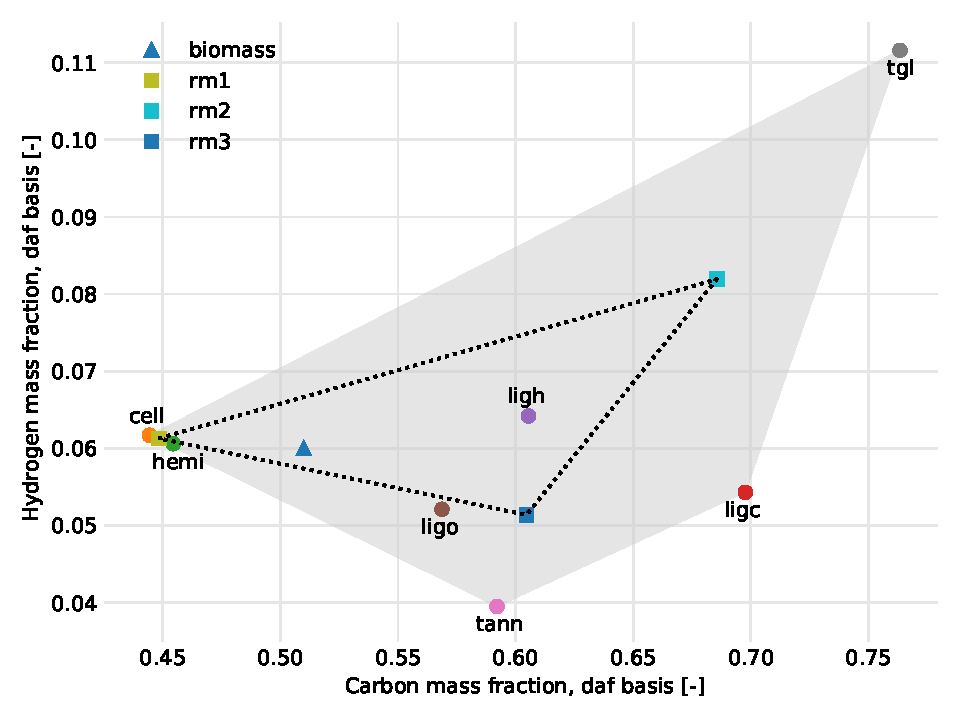
\includegraphics[width=0.8\textwidth]{figures/blend3-biocharact-ultmod.pdf}
    \caption{Characterization of the Blend3 feedstock using modified ultimate analysis data and adjusting the splitting parameters to account for extractives. Reference mixtures (rm) are labeled with square markers.}
    \label{fig:blend3-biocharact-ultmod}
\end{figure}

\textbf{Case 3:} The final approach to characterize the Blend3 feedstock, was to use chemical analysis data (see Table \ref{tab:blend3-chem-analysis}) to determine the biomass composition. Cellulose is represented by glucan while hemicellulose is comprised of arabinan, galactan, mannan, xylan, free fructose, free glucose, and sucrose. The measurement technique to determine the lignin components is unknown; therefore, the lignin is evenly divided into the carbon, hydrogen, and oxygen fractions. Tannins are represented by acetyl, water extractives, and ethanol extractives while ash is the non-structural and structural inorganics. Finally, the biomass composition based on the chemical analysis measurements is given in Table \ref{tab:blend3-biocomp}.

\begin{table}[H]
    \centering
    \caption{Biomass composition for the Blend3 feedstock. Values are reported as mass percent on a dry ash-free basis (\% daf).}
    \label{tab:blend3-biocomp}
    \begin{tabular}{lrrr}
        \toprule
        Biomass composition & Case 1 & Case 2 & Case 3 \\
        \midrule
        cellulose     & 26.38 & 39.24 & 39.19 \\
        hemicellulose & 14.33 & 25.12 & 23.26 \\
        lignin-c      & 7.84  & 8.57  & 9.89 \\
        lignin-h      & 5.27  & 3.11  & 9.89 \\
        lignin-o      & 46.18 & 18.00 & 9.89 \\
        tannins       & 0.00  & 2.95  & 7.88 \\
        triglycerides & 0.00  & 3.01  & 0.00 \\
        \bottomrule
    \end{tabular}
\end{table}

\subsection{Batch reactor conversion and yields}

Here.

\subsection{Sensitivity analysis}

Results for the sensitivity analysis of the Debiagi kinetics using a batch reactor model are shown in Tables X.

\begin{figure}[H]
    \centering
    \makebox[\textwidth][c]{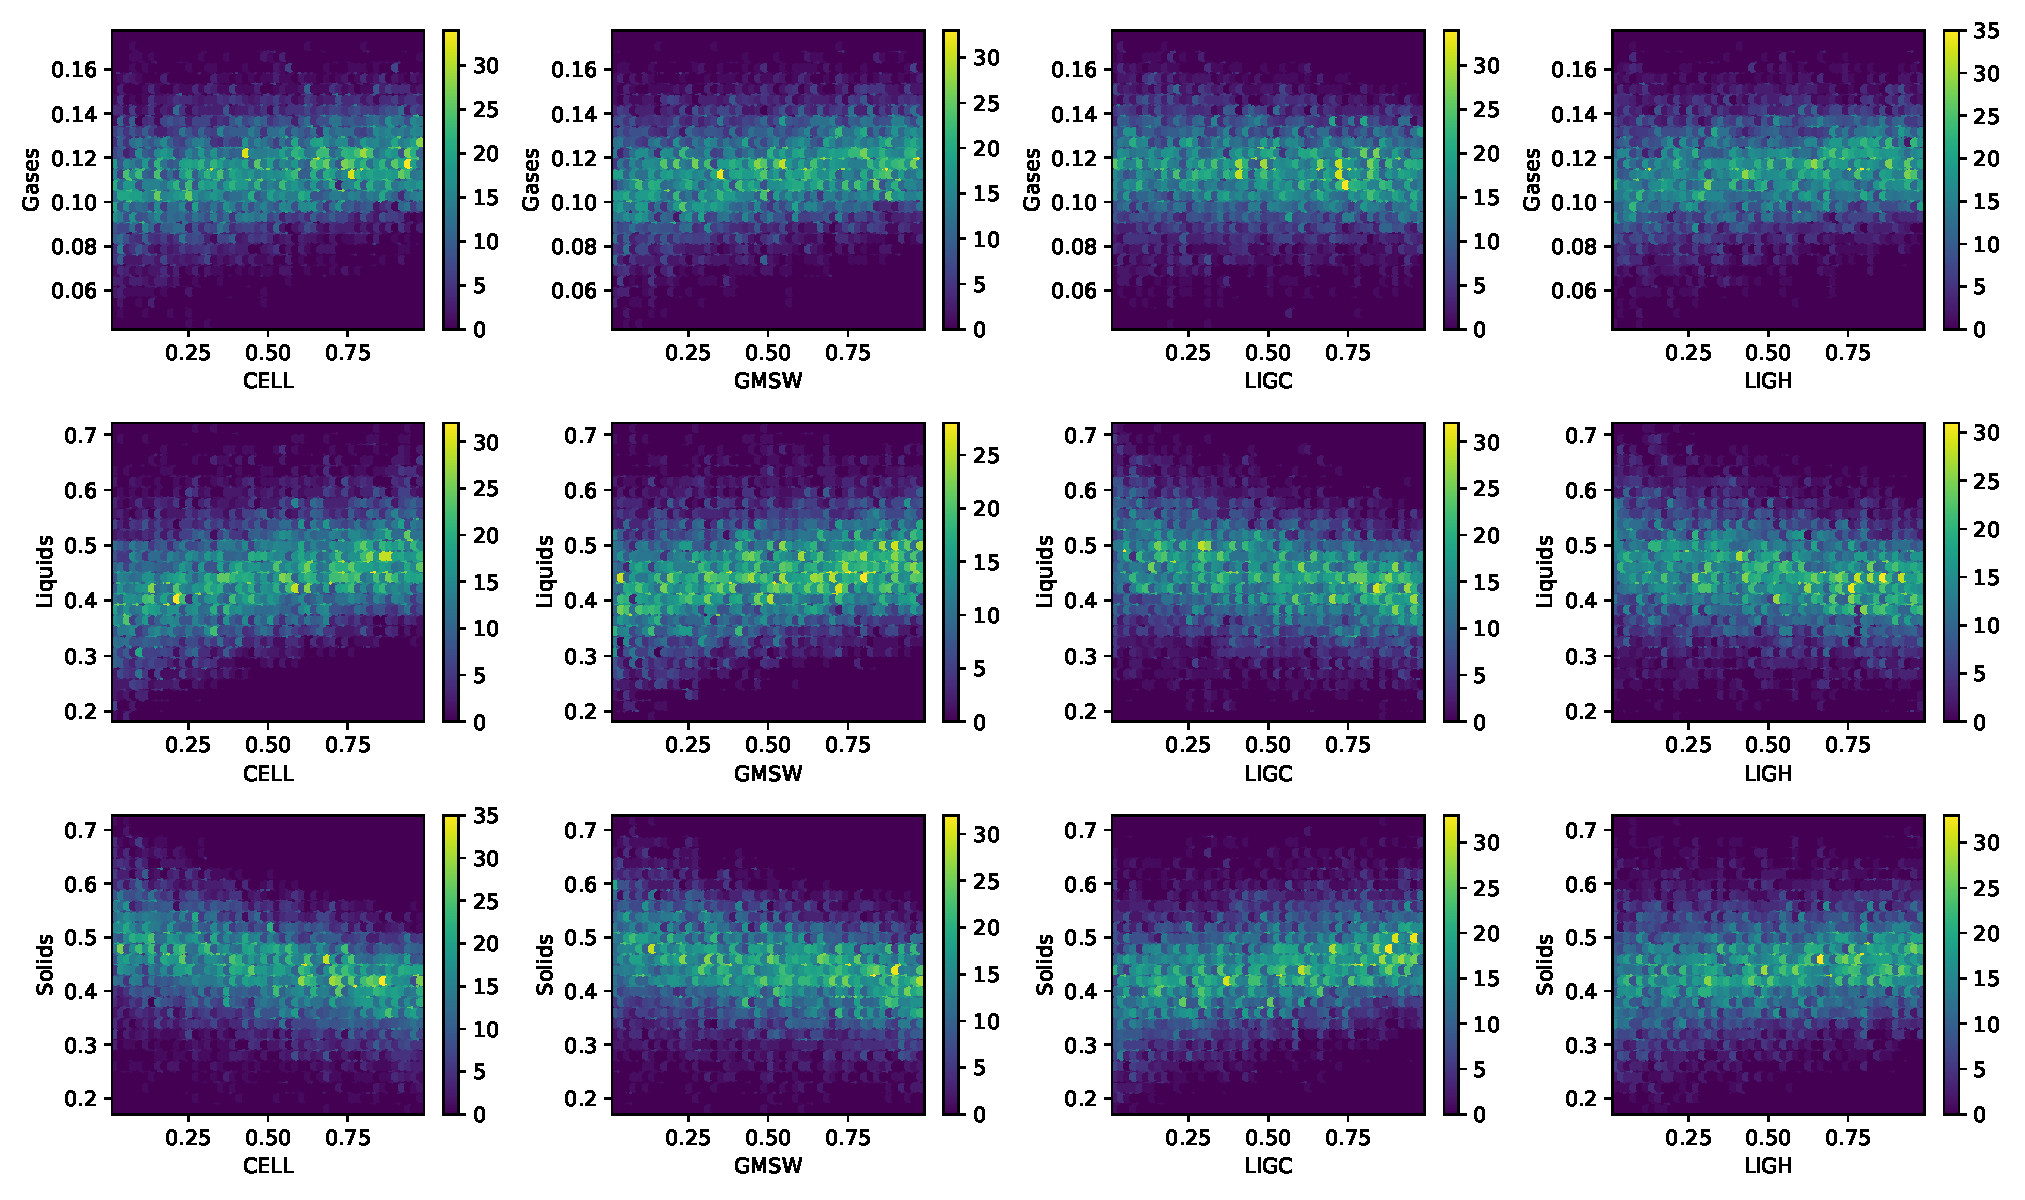
\includegraphics[width=1.3\textwidth]{figures/sa-hexbin1-n1000.pdf}}
    \caption{Batch reactor results for cellulose, hemicellulose (GMSW), carbon-rich lignin (LIGC), and hydrogen-rich lignin (LIGH) using 16,000 samples. Reaction time is 10 seconds at 773.15 K and 101,325 Pa. Colorbar represents bin count.}
\end{figure}

\begin{figure}[H]
    \centering
    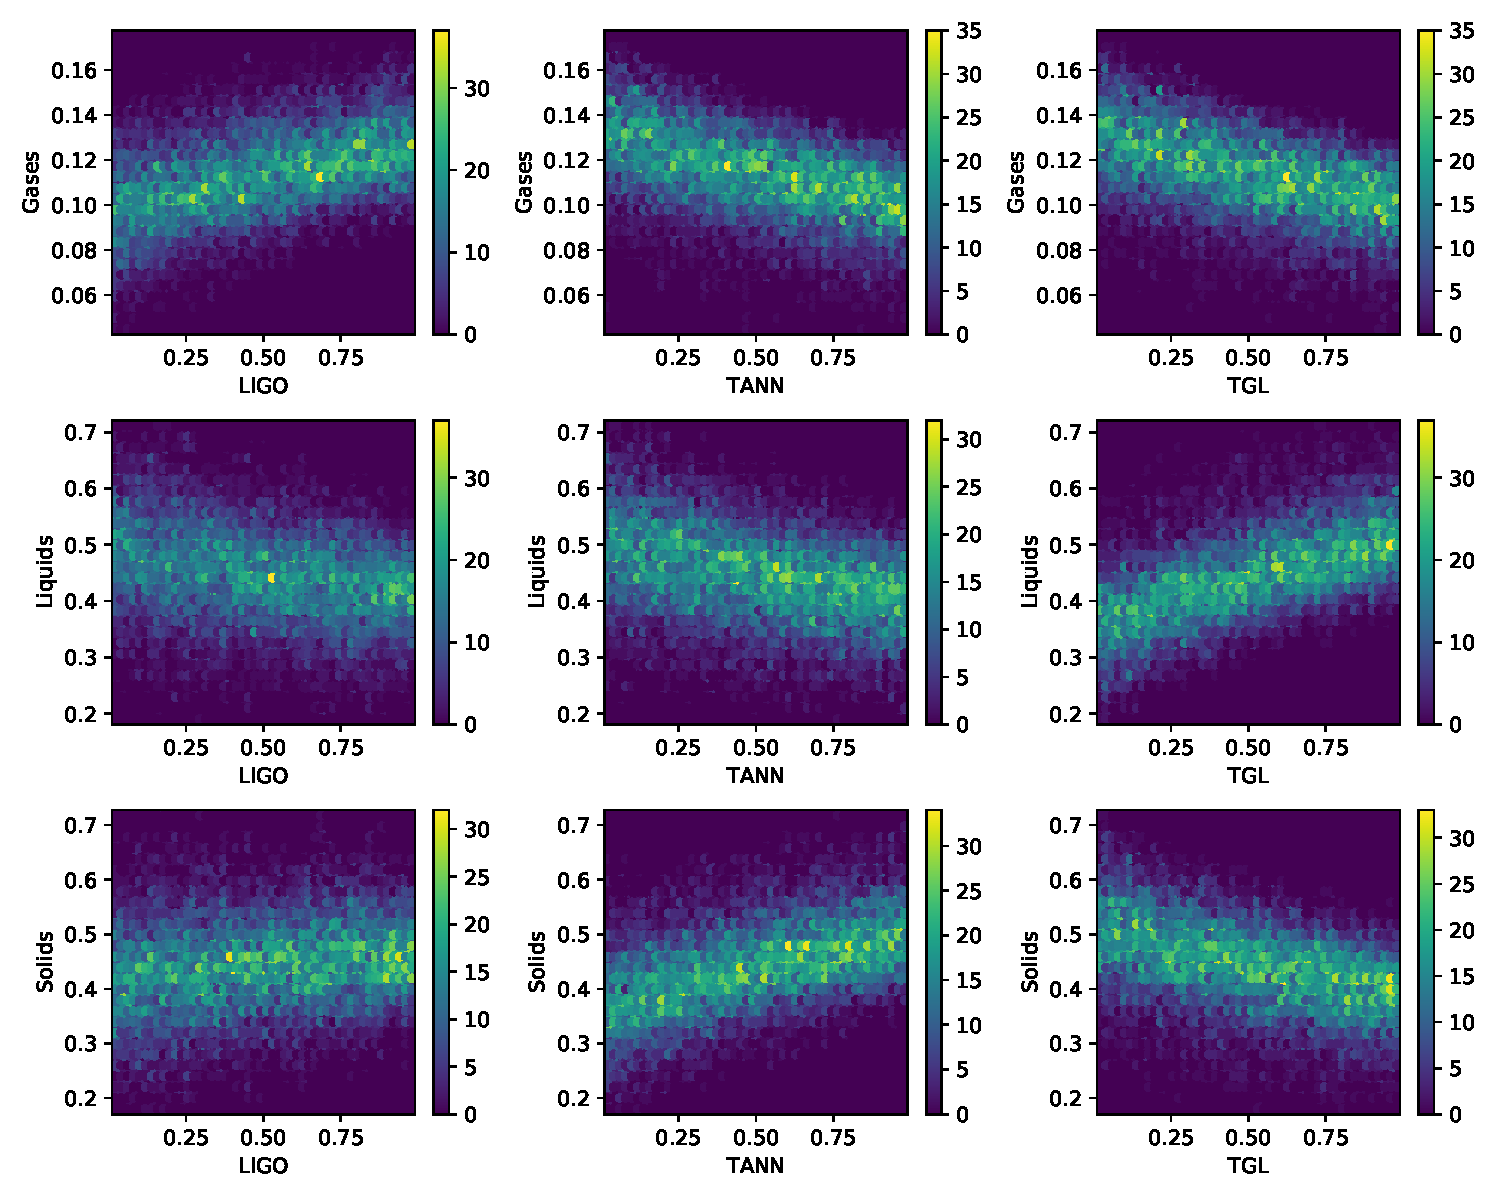
\includegraphics[width=\textwidth]{figures/sa-hexbin2-n1000.pdf}
    \caption{Batch reactor results for oxygen-rich lignin (LIGO), tannins (TANN), and triglycerides (TGL) using 16,000 samples. Reaction time is 10 seconds at 773.15 K and 101,325 Pa. Colorbar represents bin count.}
\end{figure}

\begin{figure}[H]
    \centering
    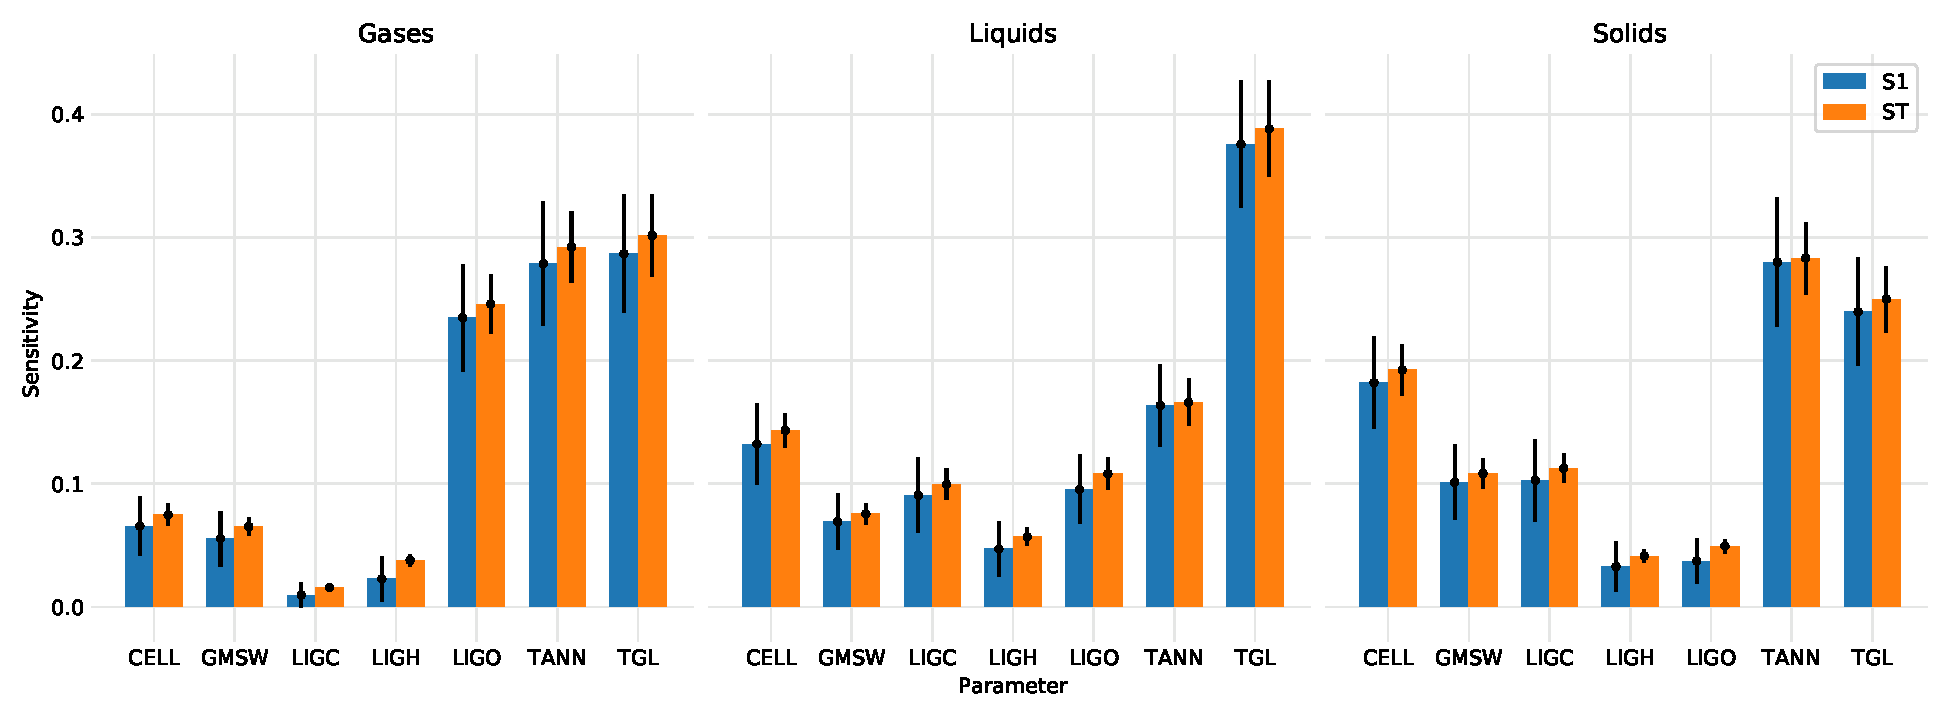
\includegraphics[width=\textwidth]{figures/sa-bar-n1000.pdf}
    \caption{First-order (S1) and total-order (ST) Sobol indices for biomass composition with reactants grouped as gases, liquids, and solids using 16,000 samples.}
\end{figure}
